
\section{Central tracking}

\subsection{Silicon microstrip tracker}

%%%%%% SLIDE
\begin{frame}{\textcolor{Goldenrod}{Silicon Microstrip Tracker}}
  \begin{overlayarea}{\textwidth}{\textheight}
    \begin{figure}[h]
      \centering
      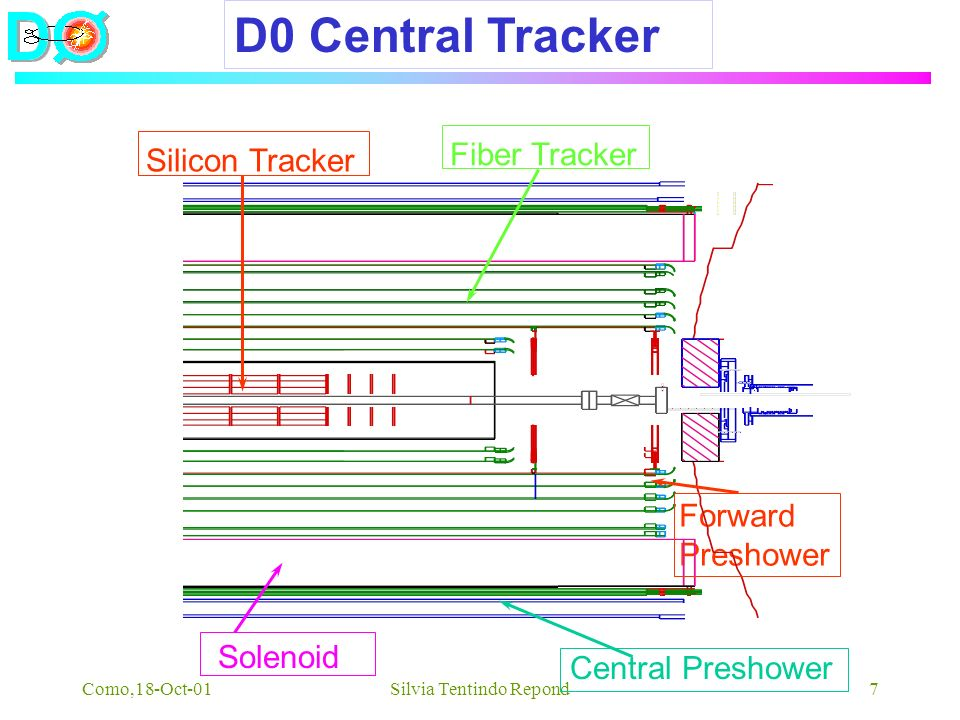
\includegraphics[height=0.5\textheight]{./Images/08_CT}
    \end{figure}

    \itt[<only@+>]
  \item
    A silicon microstrip tracker (SMT) and a central fiber tracker
    (CFT) surrounded by a solenoidal magnet

  \item
    the primary interaction vertex resolution of about $35 \mu m $
    along the beamline $\to$ \alert{ good measurement of lepton $p_T$, jet
      transverse energy ($E_T$ ), and missing transverse energy
      $\slashed{E_T}$. }\\
    \textcolor{blue}{{\small b-quark jets tagging with an impact parameter resolution of better
      than $15 \mu m$ in $r-phi$}}
    \note{for particles with transverse momentum $p_T
      > 10 GeV/c$ at $\eta = 0$.}
    \tti
  \end{overlayarea}
\end{frame}


%%%%%% SLIDE
\begin{frame}{\textcolor{Goldenrod}{Silicon Microstrip Tracker}}
  \begin{overlayarea}{\textwidth}{\textheight}
    \begin{figure}[h]
      \centering
      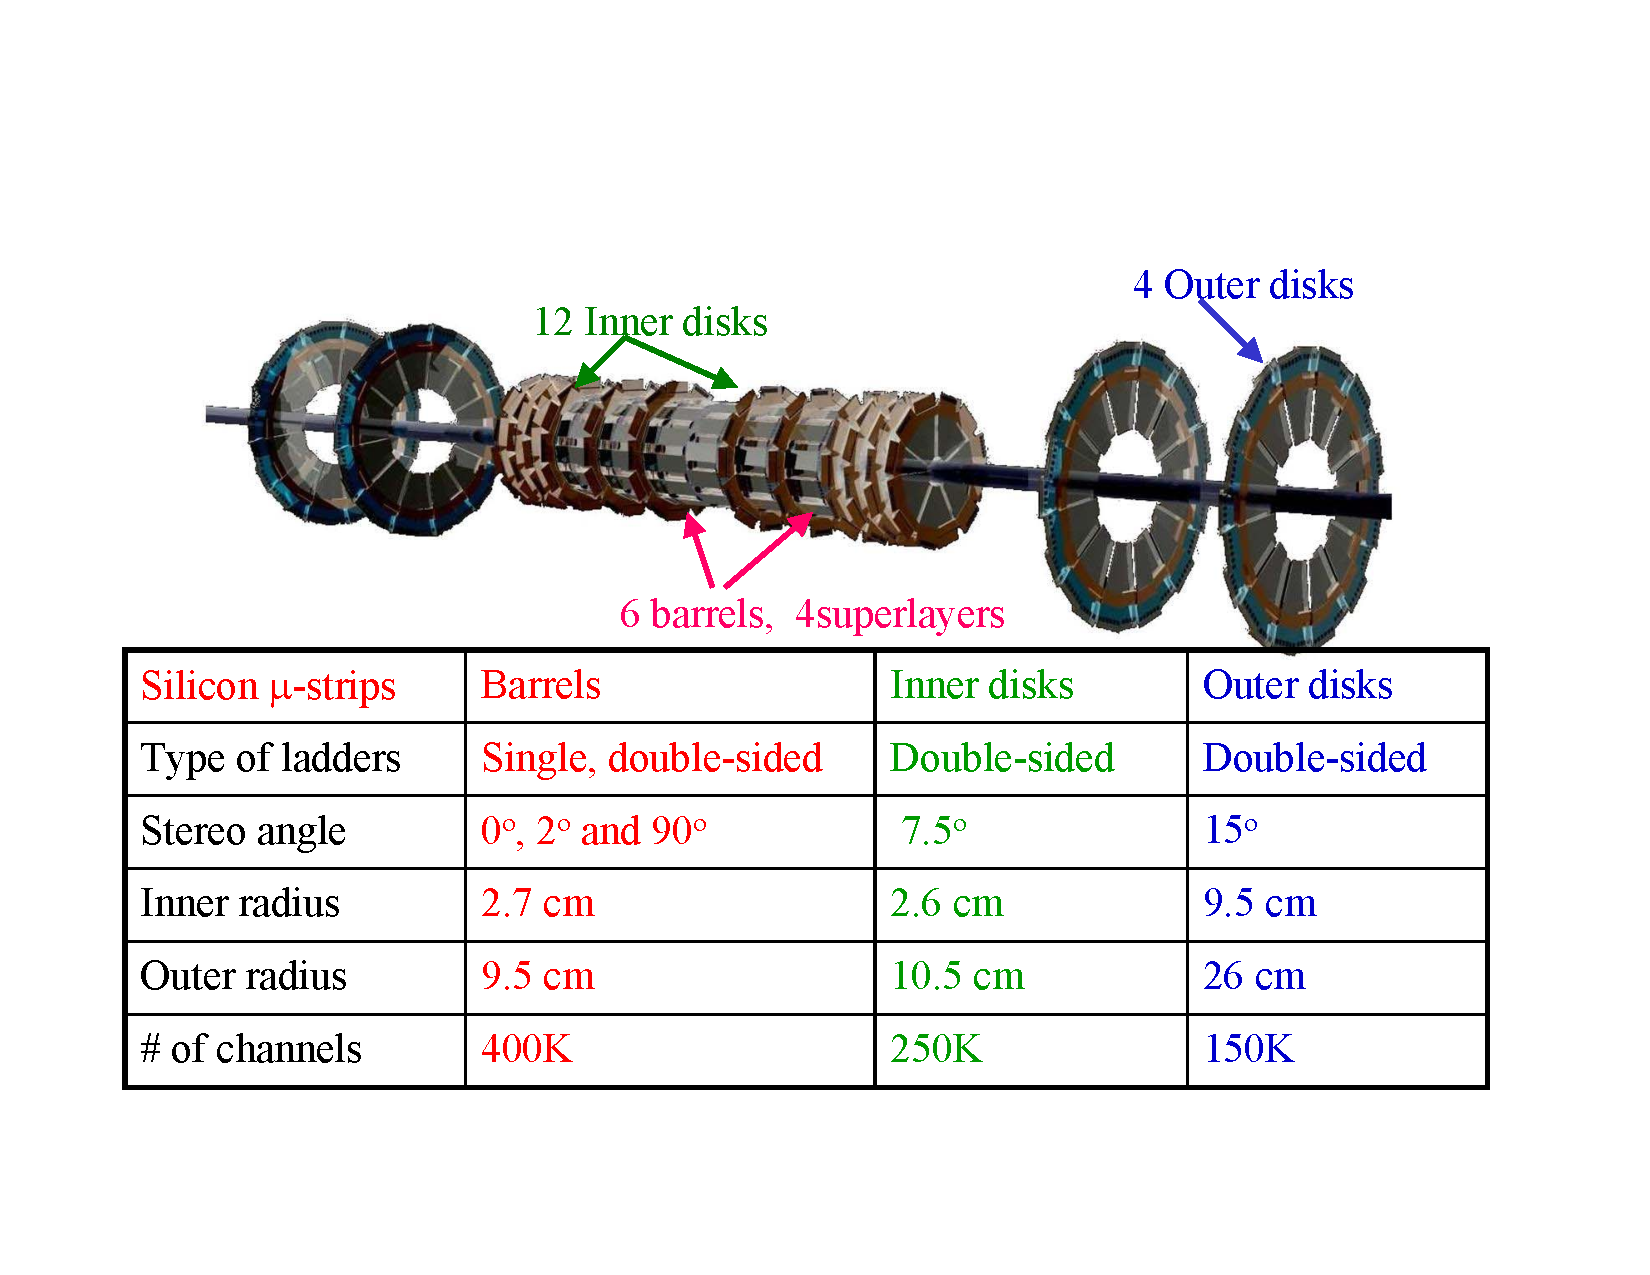
\includegraphics[height=0.4\textheight]{./Images/09_SMT}
    \end{figure}

    \itt[<only@+>]
  \item
    
 \item The SMT provides both tracking and vertexing over nearly the
   full $\eta$ coverage of the calorimeter and muon systems.
   
 \item The barrel detectors primarily measure the $r-phi$ coordinate and
   the disk detectors measure $r-z$ as well as $r-\phi$.

   
 \note{Sensor ladder assemblies were designed for low mass, pre- cise
   alignment, and good thermal performance. With the exception of the
   DSDM ladders, which use a single 12-cm sensor, ladders were
   constructed us- ing two 6-cm sensors.}
 
 \note{The SMT uses a combination of single-sided (SS), double-sided
   (DS), and double-sided double-metal (DSDM) technologies.}
 
 \note{The detector has six barrels in the central region. Each barrel
   has four silicon readout layers. The silicon modules installed in
   the barrels are called “ladders.” Layers 1 and 2 have twelve
   ladders each; layers 3 and 4 have twenty-four ladders each, for a
   total of 432 ladders.}
 
 \note{There are 144 F-wedges and 96 full H-wedges in the tracker;
   each side of a wedge (upstream and downstream) is read out
   independently. There is a grand total of 912 readout modules, with
   792,576 channels.}
 \tti
\end{overlayarea}
\end{frame}

%%%%%% SLIDE
\begin{frame}{\textcolor{Goldenrod}{Silicon Microstrip Tracker: Operation}}
  \begin{overlayarea}{\textwidth}{\textheight}
    \begin{figure}[h]
      \centering
      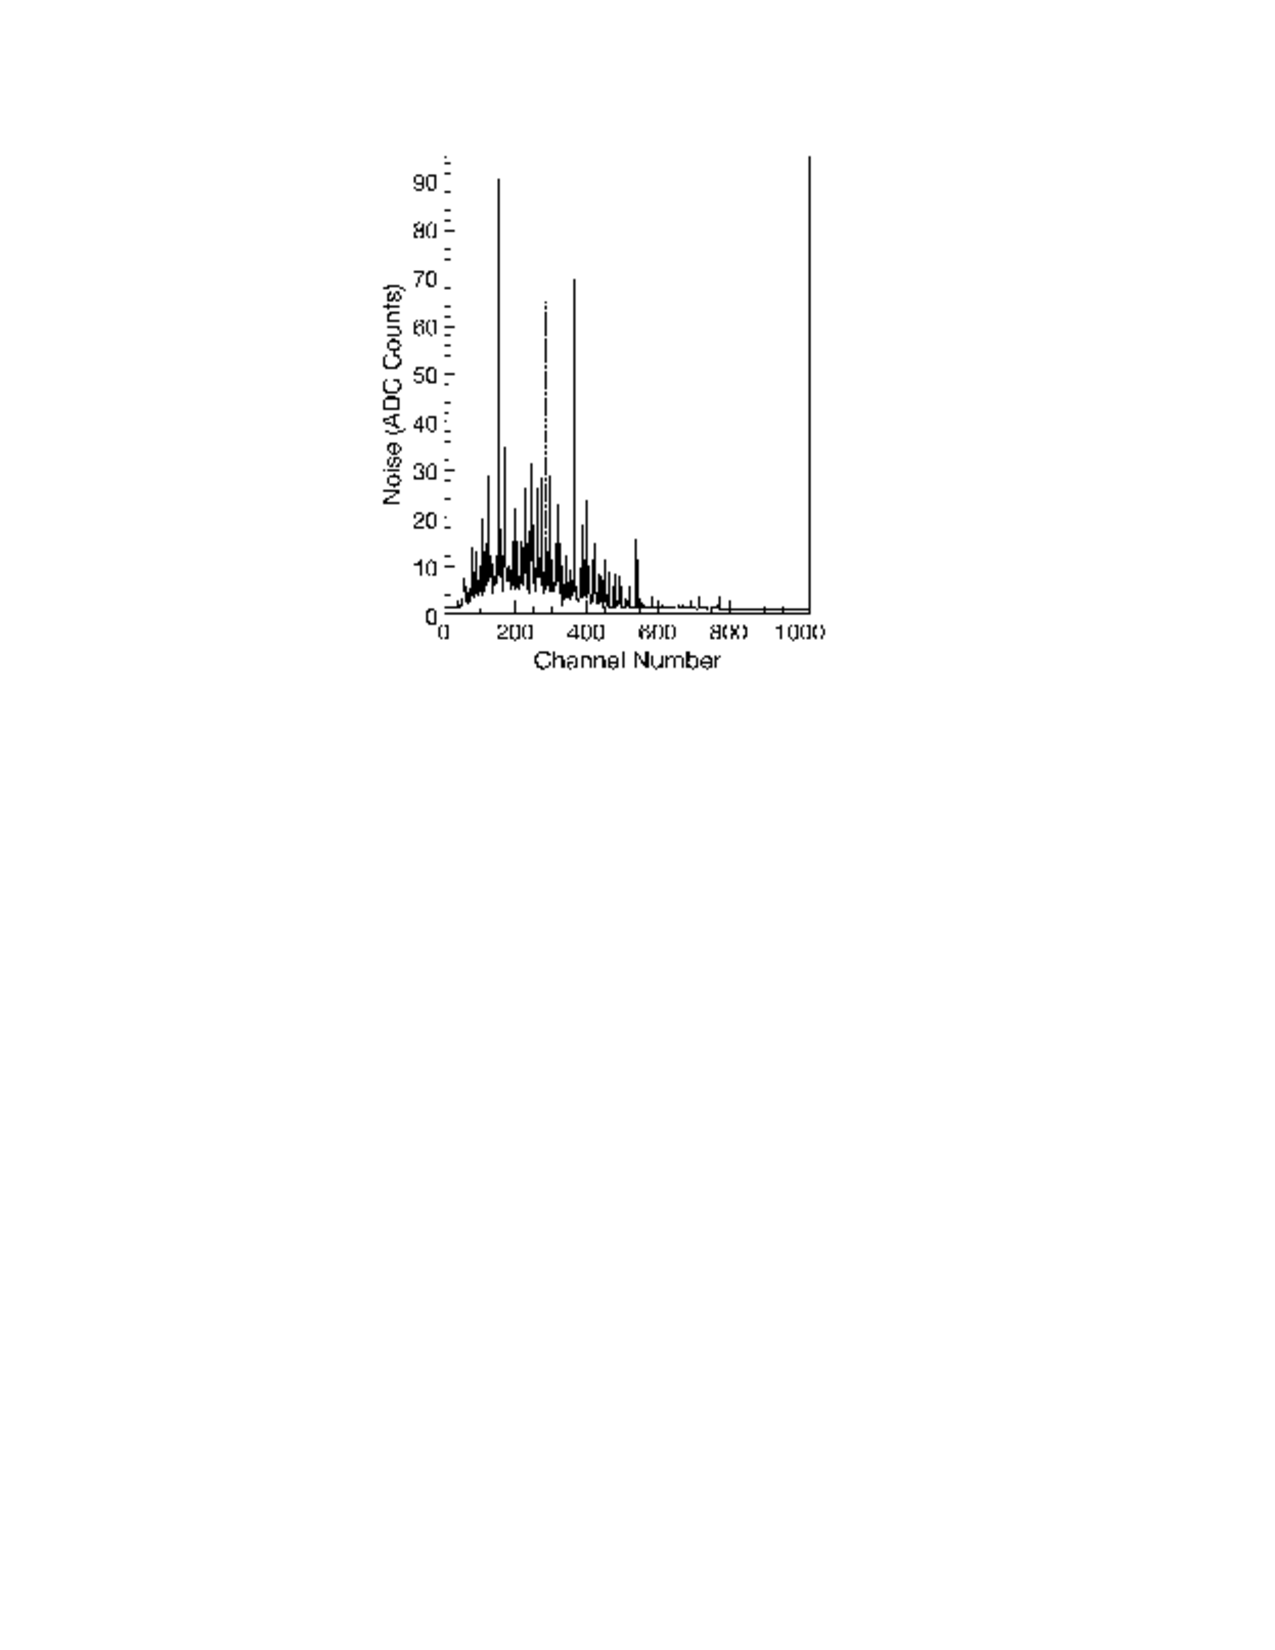
\includegraphics[height=0.4\textheight,
      width=0.45\textwidth]{./Images/11_SMT}
      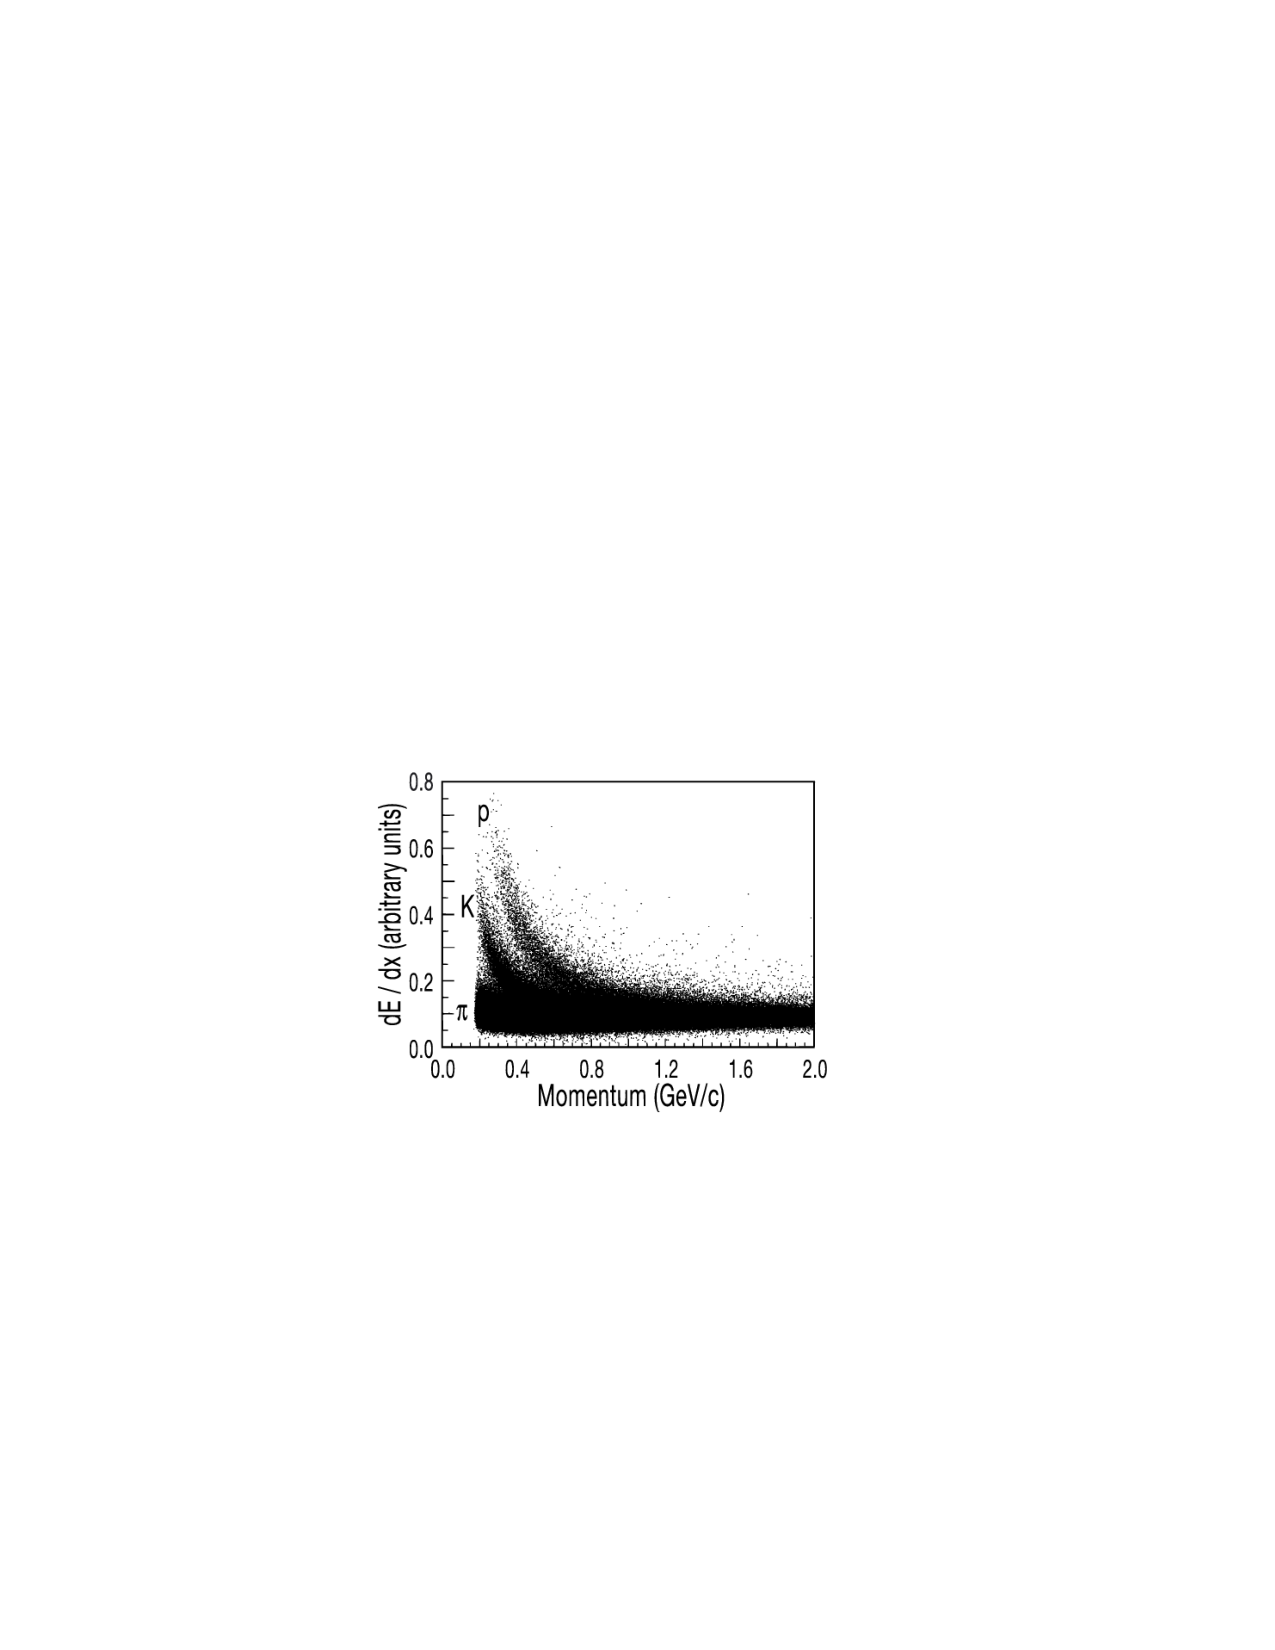
\includegraphics[height=0.4\textheight,
      width=0.45\textwidth]{./Images/12_SMT}
      \caption*{left: grassy noise seen in the Micron-supplied F-disk
        detectors. right: energy loss for a $K$-enriched sample of
        tracks showing $\pi$, $K$, and proton bands.}
      
    \end{figure}
    \itt[<only@+>]  
    
\item during run II $\approx 90$\% of sensors were functional
  
\item most operational difficulties have been peripheral to the
  silicon detector itself. These include latchup of operational
  amplifiers on the interface boards, low voltage power supply
  failures, and high leakage currents in high voltage distribution
  boxes.
  
  \note{\url{https://en.wikipedia.org/wiki/Latch-up}}
  
\item the most serious detector feature is “grassy noise,”
  which is confined to the Micron-supplied F-disk
  detectors ($75$\% of the F-disk sensors). This noise is characterized
  by large charge spikes which cover $10–20$ strips and
  occur in about $20$\% of the events for affected
  devices.
  
\item leakage currents typically rise to
  greater than $100 \mu A$ within one hour of turn-on at
  the beginning of a store.
  
\item Alignment and calibration Signal/noise performance varies with
  detector type from $12:1 to 18:1$.
  
\item Coherent noise is typically one-third
  of the random noise.
  
\item Gains vary among detector types
  with the n-sides $5–15$\% lower than the p-sides due to the larger load
  capacitance.
  \tti
  
\end{overlayarea}
\end{frame}


\subsection{Central fiber tracker}


%%%%%% SLIDE
\begin{frame}{\textcolor{Goldenrod}{Central Fiber Tracker}}
  \begin{overlayarea}{\textwidth}{\textheight}
    \begin{figure}[h]\centering
      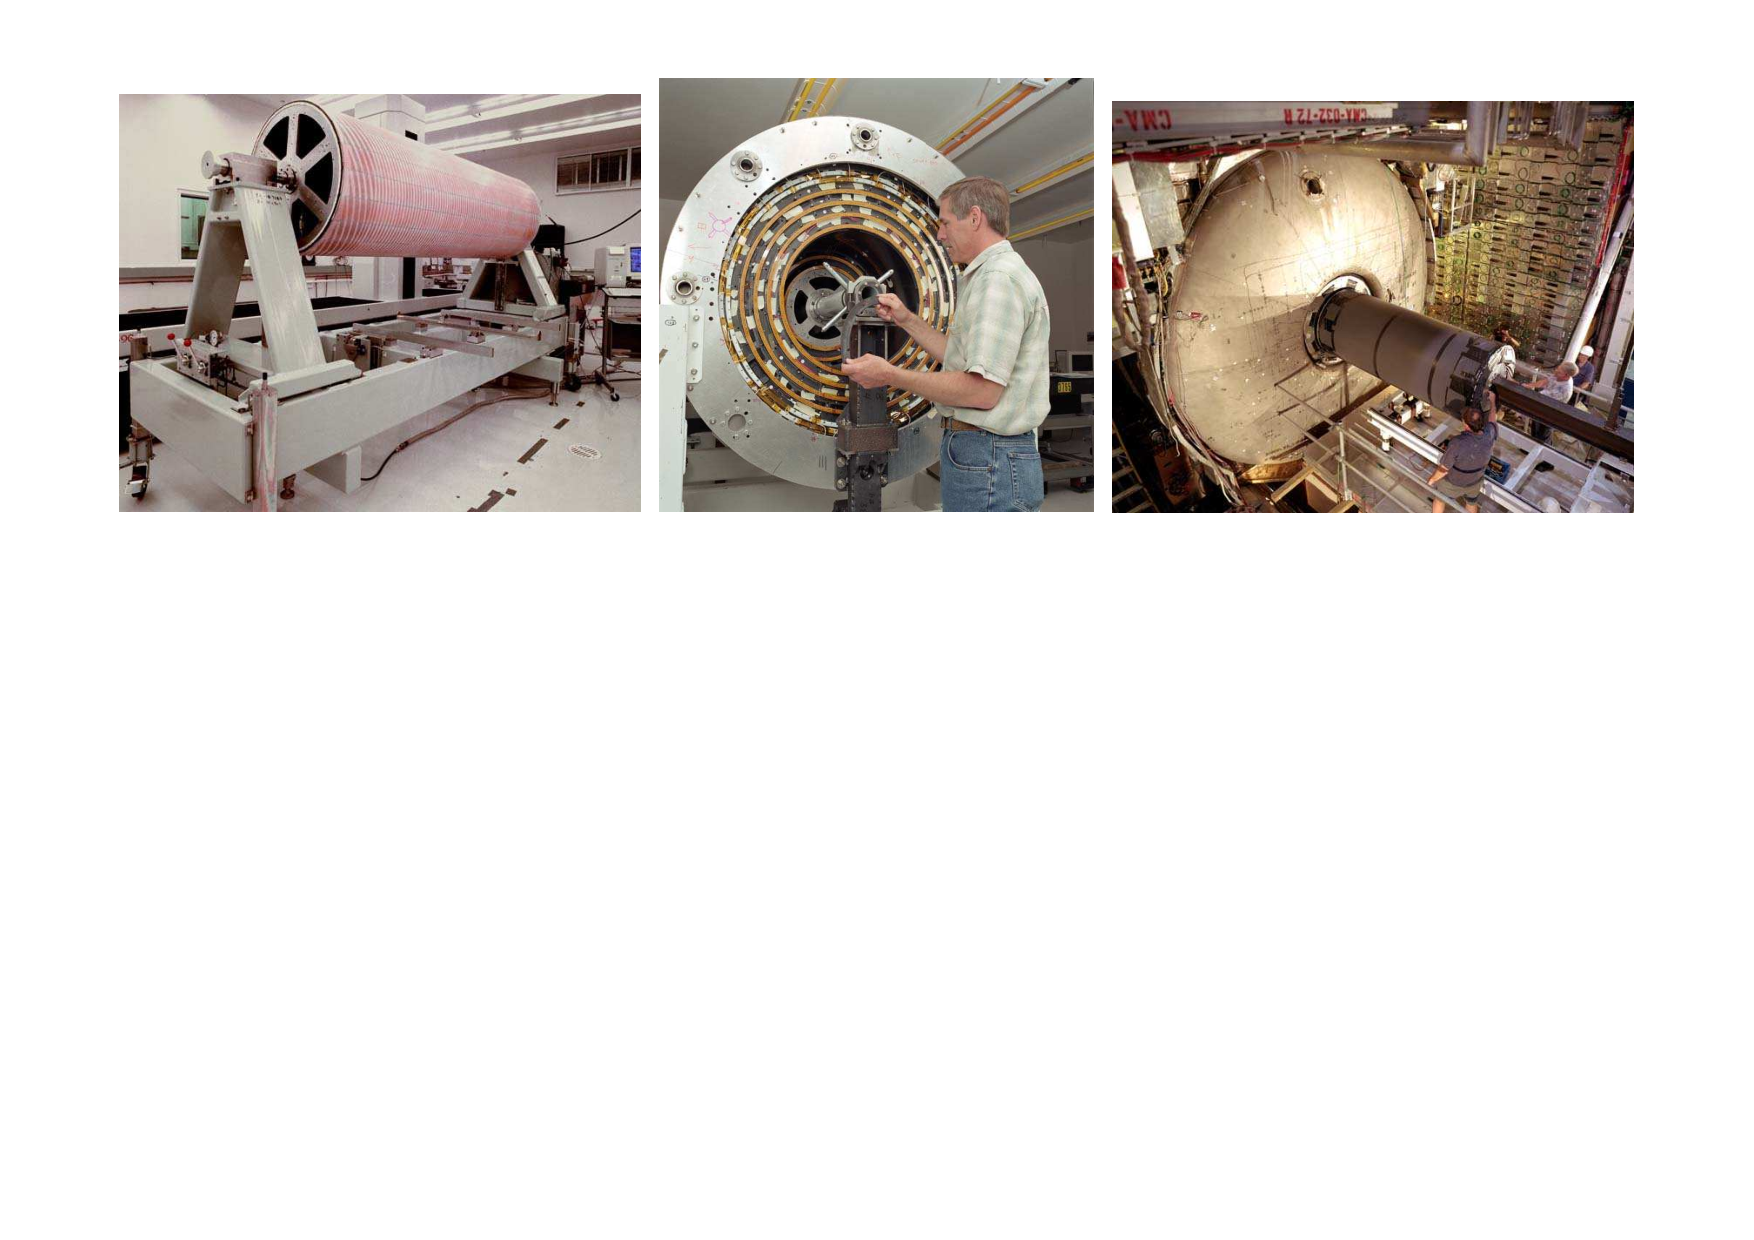
\includegraphics[height=0.3\textheight]{./Images/13_CFT}
    \end{figure}
    \itt[<+->]  

    \note{scintillating fibers mounted on eight concentric
      support cylinders ($20 to 52 cm$ from
      the center of the beampipe. The
      two innermost cylinders are $1.66 m$ long; the outer six cylinders are
      $2.52 m$ long.}
      
    \note{ Each cylinder supports one doublet layer of fibers oriented
      along the beam direction and a second doublet layer at a
      stereo angle in $\phi$ of $+3^{\textdegree}$.}
    
    \item 8 coaxial carbon cylinders, each supporting 2 doublet layers
      on their outside surface
    \item 8 axial layers are formed by fibers oriented along the
      cylinder
    \item 4 stereo layers are formed by fibers oriented at $+3^{\textdegree}$ and 4 stereo
      layers at $-3^{\textdegree}$
    \item Position resolution of fiber doublet is $\approx 100 \mu m$
      \tti
\end{overlayarea}
\end{frame}

%%%%%% SLIDE
\begin{frame}{\textcolor{Goldenrod}{Central Fiber Tracker: fibers}}
  \begin{overlayarea}{\textwidth}{\textheight}
    \begin{figure}[h]\centering
      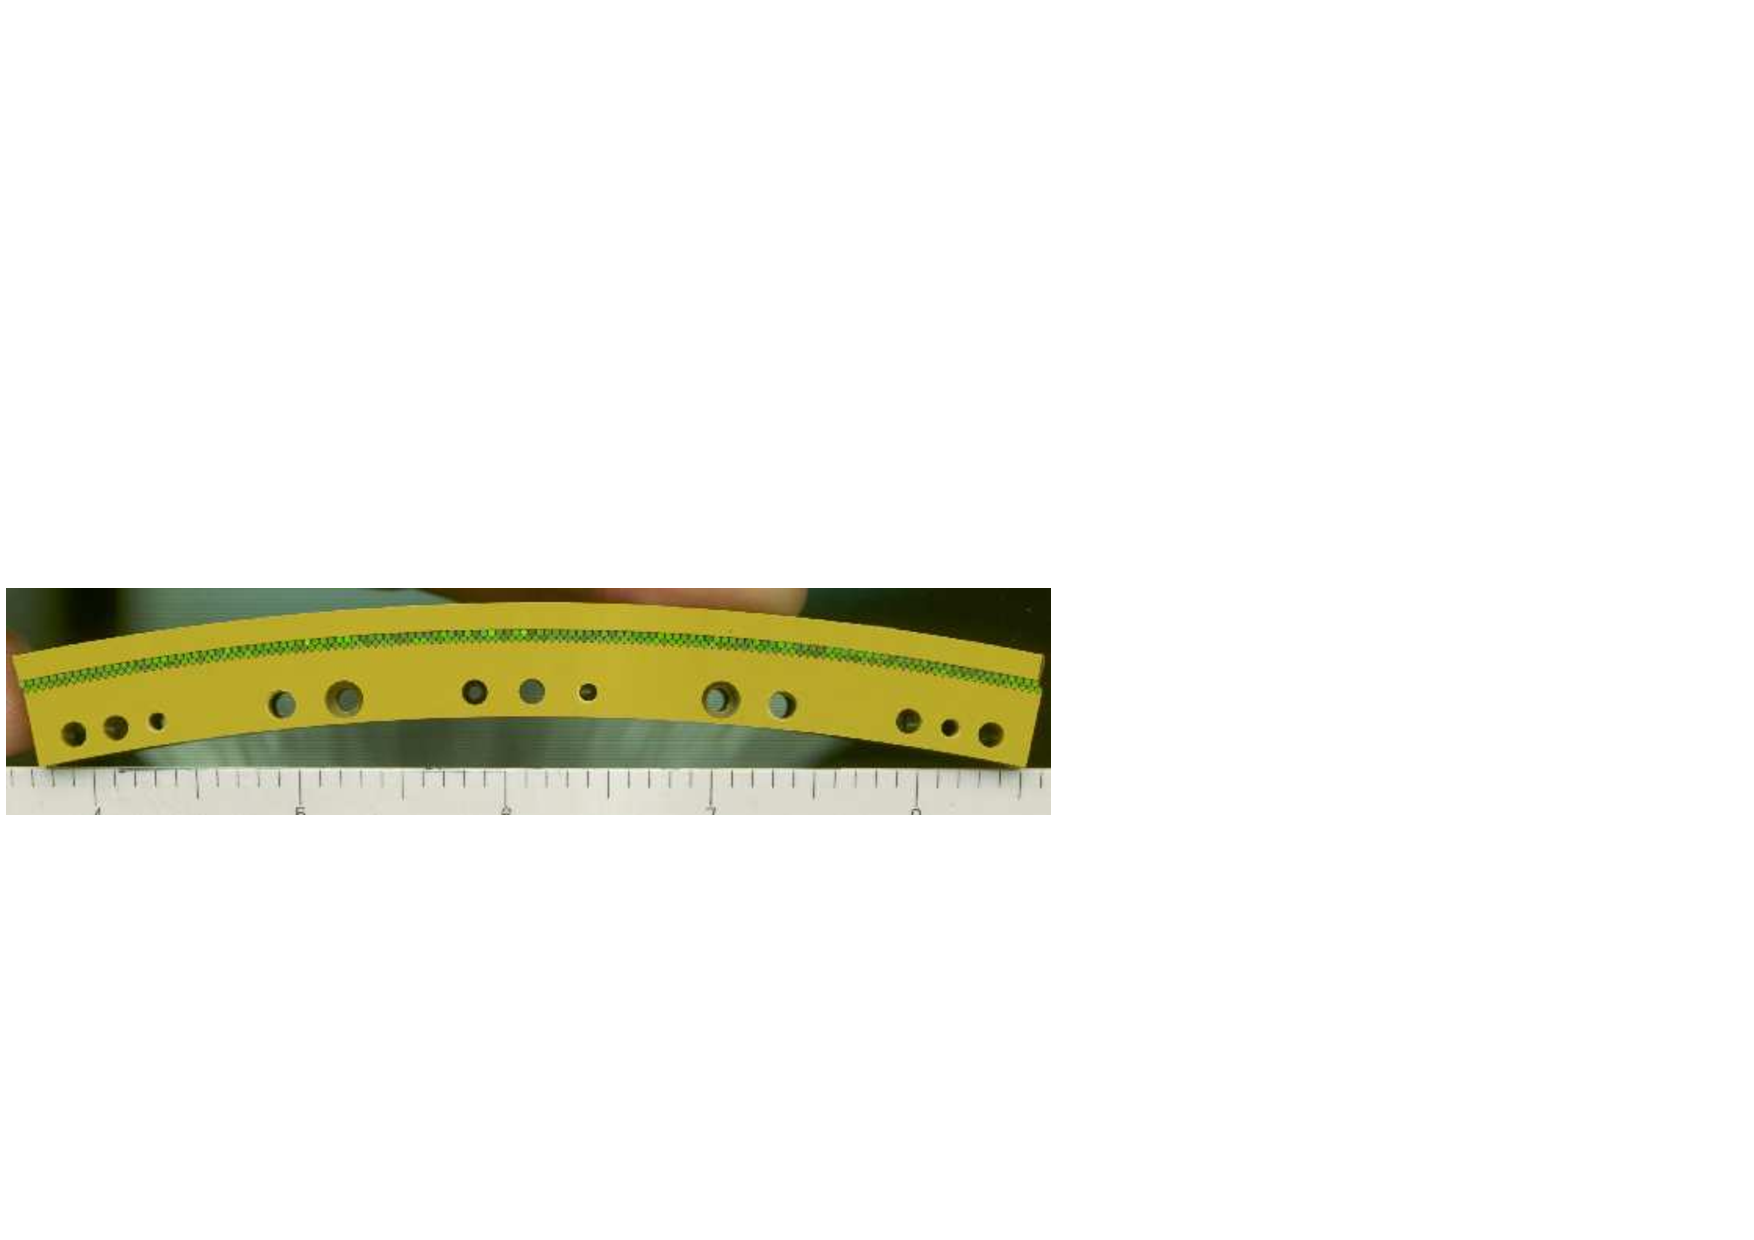
\includegraphics[height=0.3\textheight, width=0.6\textwidth]{./Images/15_CFT}
      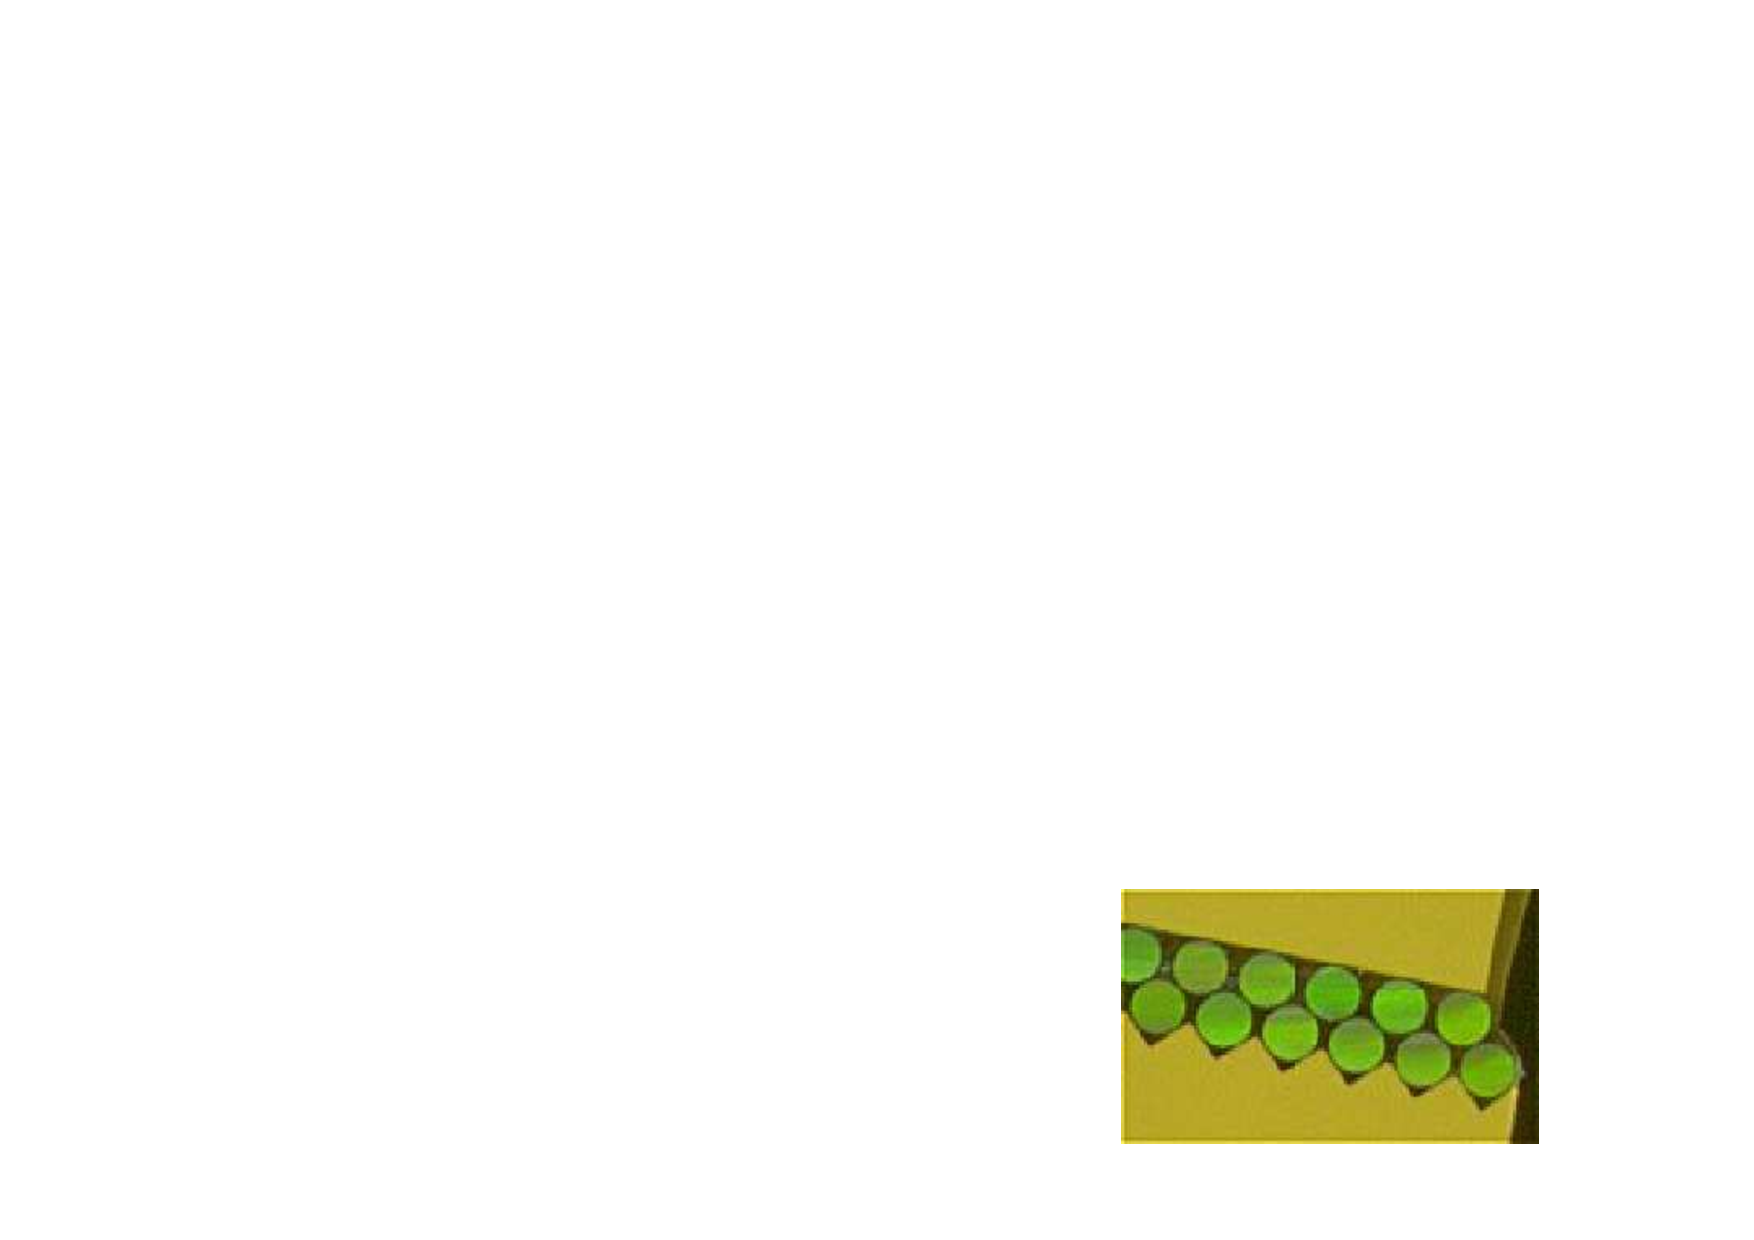
\includegraphics[height=0.3\textheight, width=0.3\textwidth]{./Images/16_CFT}
    \end{figure}
    \itt[<only@+>]

  \item  $d = 835 \mu m \times h =1.66/2.52 m$ scintillation fibers are 
    connected to clear fiber waveguides of identical diameter ($7.8 to 11.9 m$ long)
    
  \item light production: The base core material is polystyrene (PS). The PS is
    doped with the organic fluorescent dye paraterphenyl (pT) to
    about 1\% by weight.
  \item excitations in the PS are rapidly transferred to the pT via a
    non-radiative dipole-dipole interaction.
    
  \item a 3-hydroxyflavone (3HF) wave-shifter, is used to
    transmit the $340 nm \to 530 nm$
  \item The scintillating fibers were assembled into ribbons
    consisting of 256 fibers in two layers of 128 fibers each.
    \tti
  \end{overlayarea}
\end{frame}


%%%%%% SLIDE
% \begin{frame}{\textcolor{Goldenrod}{Central Fiber Tracker}}
%   \begin{overlayarea}{\textwidth}{\textheight}
%     \begin{figure}[h]\centering
      
%     \end{figure}
%     \itt[<only@+>]
    
%   \item[$\Box$] Mechanical support structure:\\
%     \itt
%   \item The eight support cylinders are each double-walled with a
%     0.25”-thick core of Rohacell [59].
    
%   \item The walls are constructed
%     from linear carbon fibers impregnated with about 40\% resin.
    
%   \item
%     Successive cylinders are nested together by thin carbon-fiber
%     annular rings that connect the inner surface of the end ring of
%     one cylinder to a carbon-fiber ring mounted on the outer fiber
%     surface of the cylinder immediately inside.
    
%   \item For tracks traversing the detector at normal incidence, the
%     thickness of each cylinder can be described as follows: 0.28\% of
%     a radiation length for the scin-
%     tillating fibers, 0.32\% for the
%     carbon fiber support cylinder, 0.13\%
%     for the glue used to make ribbons
%     out of fibers, and 0.17\% for the
%     glue used to attach the ribbons to
%     the support cylinders.
%     \tti
    
%     \tti
%   \end{overlayarea}
% \end{frame}


%%%%%% SLIDE
\begin{frame}{\textcolor{Goldenrod}{Central Fiber Tracker: VLPC}}
  \(
  \<{0.3\textwidth}
  \img{21_CFT_VLPC.jpg}\\
  \img{21_CFT_VLPC_01.jpg}\\
  \img{21_CFT_VLPC_02.jpg}\\
  \>
  \<{0.7\textwidth}
  \itt[<+->]
\item Visible Light Photon Counter (VLPC) is a solid state photo-detector with $8$ input pixels $1
  mm$ in diameter each
\item VLPC is operated at $9 K$ with bias voltages $6-8 V$
\item provides high gain of $25000-60000$ electrons per detected
  photon
\item VLPCs with similar properties grouped together to optimize
  performance
  \tti
  \>
  \)
\end{frame}


%%%%%% SLIDE
\begin{frame}{\textcolor{Goldenrod}{Central Fiber Tracker: Central Track Tigger (CTT)}}
  \(
  \<{0.7\textwidth}
  \itt[<+->]
\item Counts track candidates identified in axial view of CFT by
  looking for hits in all 8 axial layers
\item Combines tracking and preshower information to identify
  electron and photon candidates
\item
  Generates track lists allowing other trigger systems to
  perform track matching
  \tti
  \>
  \<{0.3\textwidth}
  \img{20_CFT}
  \>
  \)
\end{frame}

%%%%%% SLIDE
\begin{frame}{\textcolor{Goldenrod}{Central Fiber Tracker: performance}}
  \begin{overlayarea}{\textwidth}{\textheight}
    \begin{figure}[h]\centering
      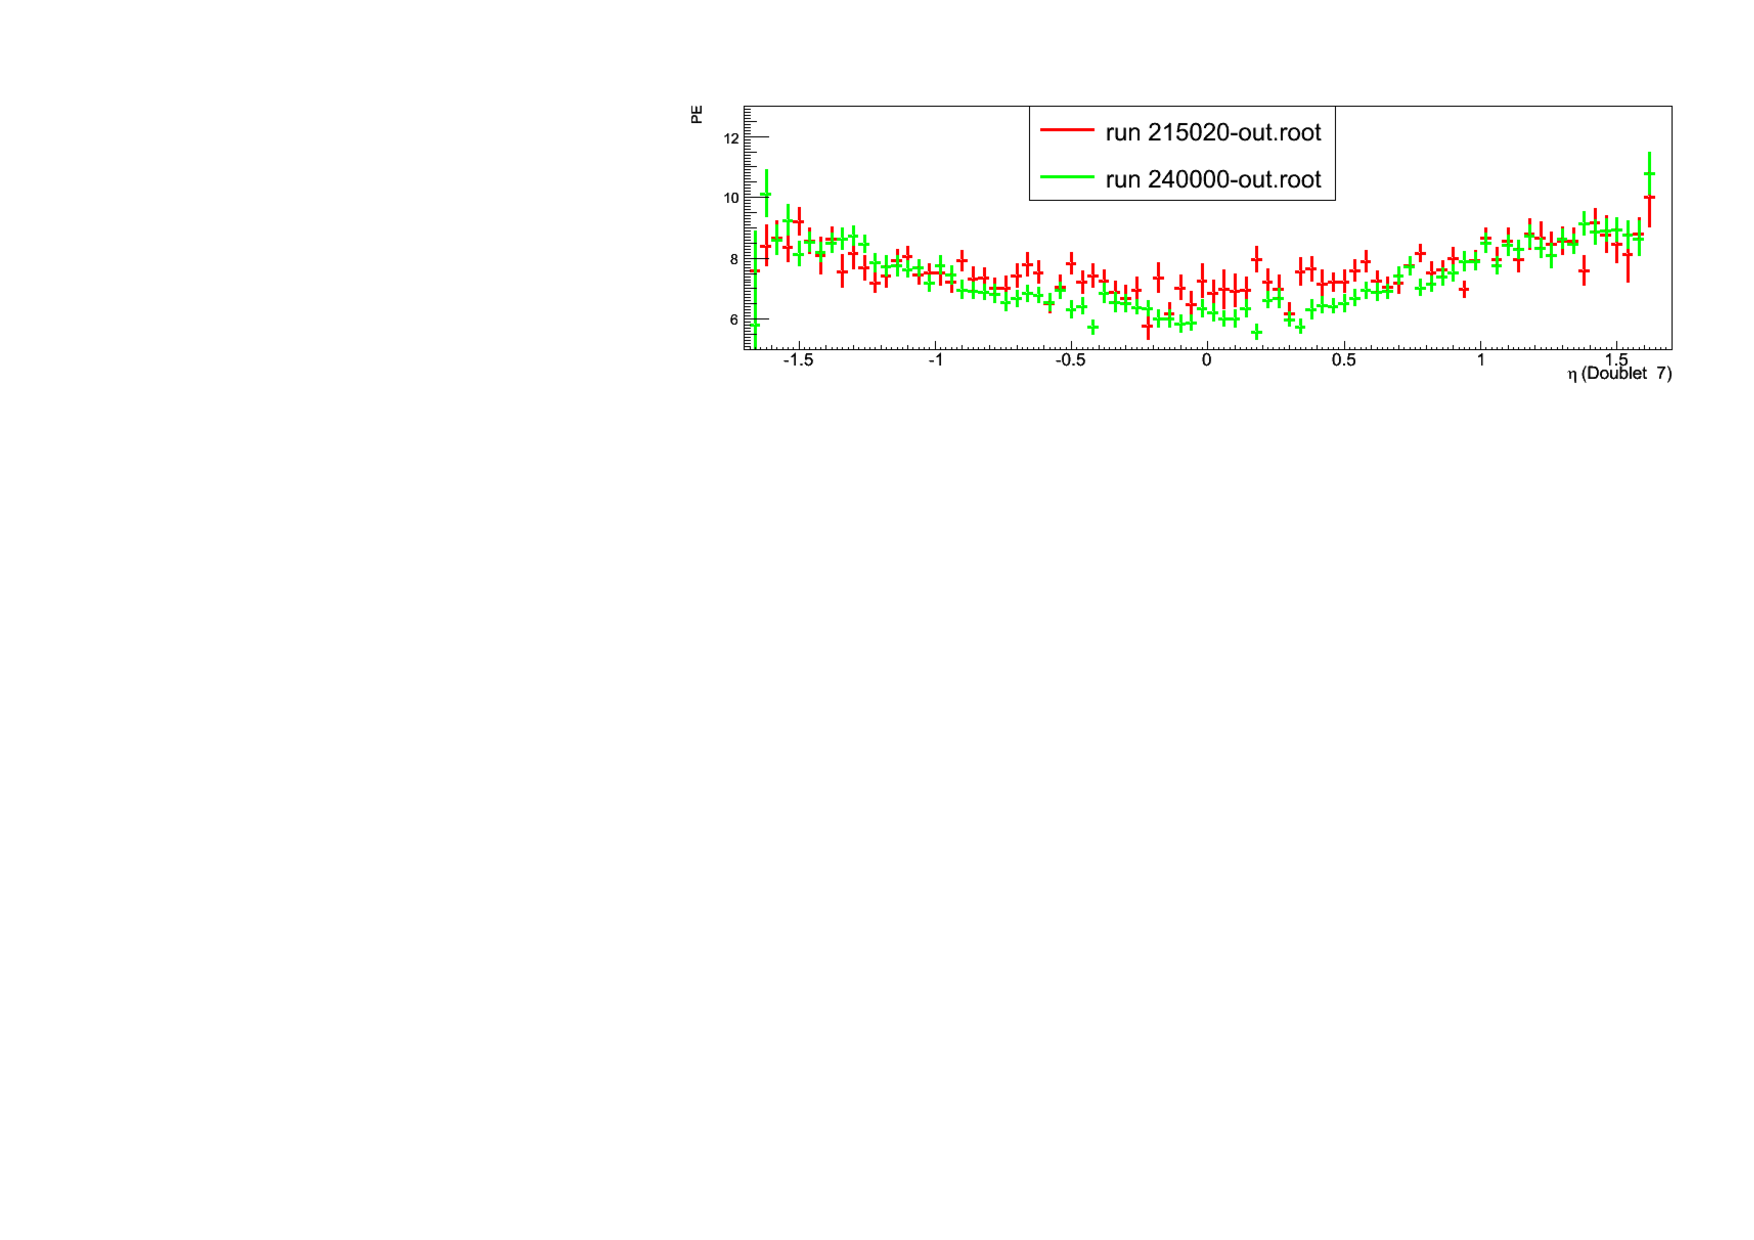
\includegraphics[height=0.2\textheight]{./Images/22_CFT_performance.pdf}\\
      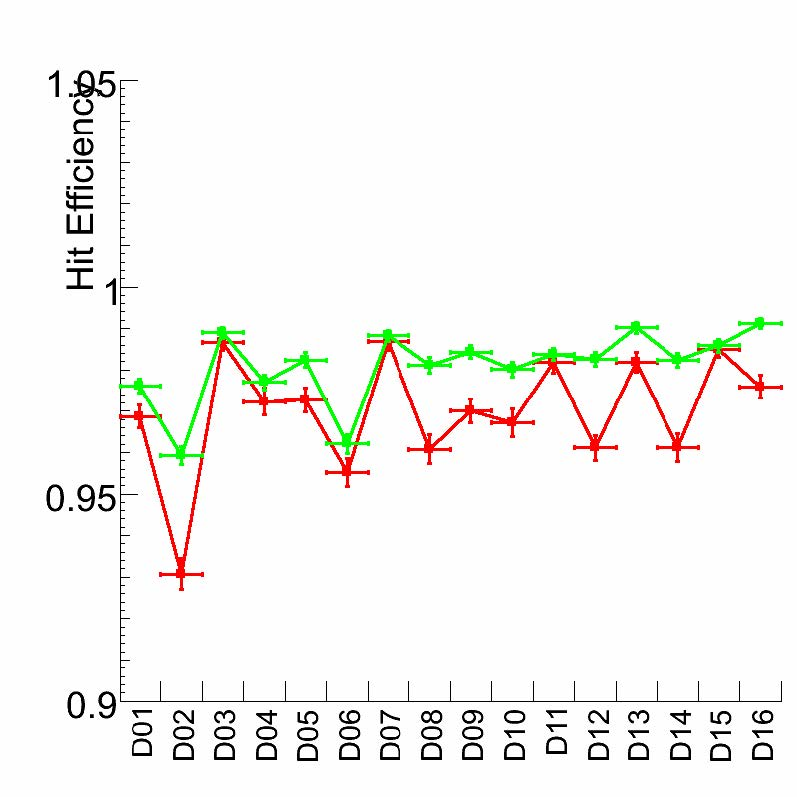
\includegraphics[height=0.2\textheight]{./Images/23_CFT_performance}
      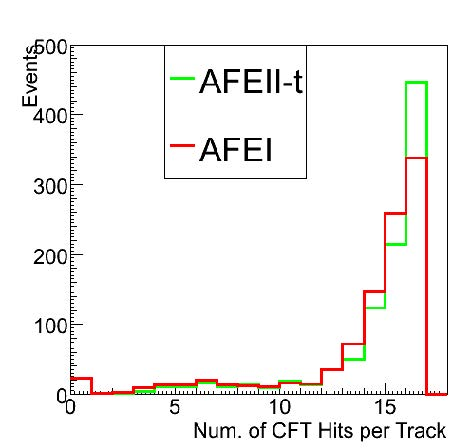
\includegraphics[height=0.2\textheight]{./Images/24_CFT_performance}
    \end{figure}
    \itt[<+->]
  \item Average light yield depends upon path length through
    scintillator.
  \item On average 8 photons produced per hit
  \item Using good 15 hit CFT tracks, the average probability of a
    cluster in excluded layer is $98$\%
    \tti
 \end{overlayarea}
\end{frame}